% Number 921
% CAPMA Algebra  Units 
% Rocket upwards - max. v, h? Algebraic
% JG

% Watermark
\AddToShipoutPicture*{\BackgroundPic}

\addtocounter {ProbNum} {1}

%\begin{floatingfigure}[r]{.44\textwidth}
%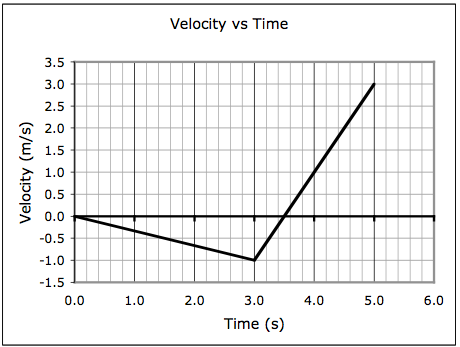
\includegraphics[scale=.54]{/Users/jgates/desktop/latex/pics/vgraph6}
%\end{floatingfigure}
 
{\bf \Large{\arabic{ProbNum}}} A rocket launches and travels upwards with an acceleration of ${4.5~\tfrac{m}{s^2}}$ for 6 seconds; at that point it runs out of fuel and goes into freefall.   \bigskip

Determine the rocket's maximum speed on the upwards trip and amount of time that it will take for it to hit the ground (from launch to impact).  \vfill


%\begin{center}
%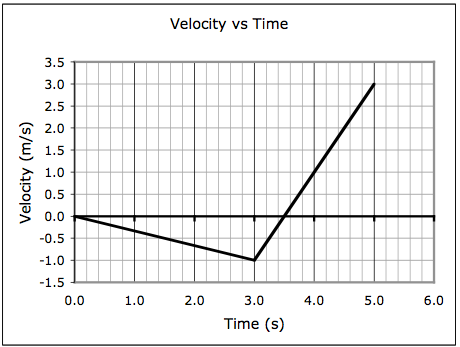
\includegraphics[scale=1]{/Users/jgates/desktop/latex/pics/vgraph6}
%\end{center}


\newpage